\documentclass[9pt,twocolumn,twoside,lineno]{style}

\articletype{NEI} % article type

\title{Resenhas 04: \textit{The Economic Institutions of Capitalism} (Williamson 1985)}
\date{17 de abril de  2020}

\author[$\ddagger$]{Gabriel Petrini}

\affil[$\ddagger$]{Doutorando no instituto de Economia da Unicamp}

\keywords{Keyword \\ Keyword2 \\ Keyword3 \\ ...}

\runningtitle{Resenhas 03} % For use in the footer 

%% For the footnote.
\runningauthor{Petrini}

\begin{abstract}
\end{abstract}

\begin{document}

\maketitle\articletypemark
\marginmark
\thispagestyle{firststyle}
\section{Introdução às instituições e à mudança institucional}

\autor abre o capítulo definindo instituições como as regras do jogo, ou ainda, como restrições humanamente concebidas que moldam a interação humana. Em seguida afirma que mudanças institucionais determinam a forma que as sociedade evoluem ao longo do tempo e, portanto, são centrais para compreender a mudança histórica. Além disso, pontua que não existe um constructo teórico que integra uma análise institucional na teoria e na história econômica.

\subsection{I}

De modo geral, as instituições diminuem a incerteza ao prover uma estrutura a vida cotidiana e por guiar as interações humanas. Em seguida, categoria instituições em formais e informais em que regras são exemplos das primeira enquanto convenções e códigos de conduta são exemplos da segunda. Também destaca que as instituições podem ser criadas e evoluir ao longo do tempo. Pontua a dimensão negativa (restrição de ações) quanto positiva (permissividades) das instituições, ou seja, envolvem as interações humanas. Adiante, diferencia instituições de \textbf{organizações} em que as segundas surgem como consequência do --- e influenciam o --- arranjo institucional e incluem grupos políticos, econômicos, sociais e educacionais em que tais agrupamentos possuem objetivos em comum.
Outra distinção relevante é entre agentes e as regras/normas (jogadores das regras).

Adiante, \autor discute que as instituições são criadas e alteradas pelos humanos de modo a teoria institucional que propõe deve partir do \textbf{nível individual}.
Também pontua que as instituições determinam o desempenho econômico ao afetar os custos de produção.

\subsection{II}

Mais uma vez, o autor retoma que instituições reduzem as incertezas de uma sociedade ao promover uma estrutura estável às interações humanas, mas tal estabilidade não implica imutabilidade. Argumenta que as mudanças institucionais são complexas uma vez que podem ser consequências de mudanças formais, informais e nas formas de execução. Pontuam que as instituições informais estão menos sujeitas à ações políticas do que as formais. Dito isso, direciona a discussão para as condições que levam a uma maior convergência ou divergência das sociedades\footnote{Afirma que abandonou a explicação via incentivos de preços antes defendida em outro livro.}. Defende que a resposta a esse questão se dá pela interação entre instituições e organizações assim como na determinação de oportunidades associadas ao arranjo institucional em que as organizações são criadas para extrair vantagens dessas oportunidades e, na medida que se altera, modificam as instituições. 

Argumenta que a trajetória da mudança institucional é determinado pelo \textit{lock-in} derivado da relação entre instituições e organizações e pelos \textit{feedbacks} dos agentes. Destaca ainda que as mudanças institucionais (incrementais) decorrem da percepção dos agentes das organizações políticas e econômicas podem ser favorecidos ao alterar o arranjo institucional na margem. No entanto, esta percepção depende da obtenção e processamento dessas informações. Em seguida, destaca que custos de transação (políticos e econômicos) tornam os \textbf{direitos de propriedade} ineficientes, mas a racionalidade limitada dos agentes tornam tais direitos de propriedade persistentes.

\autor afirma também que as mudanças institucionais podem tanto melhorar quanto piorar o bem-estar econômico. À luz disso, defende que o sucesso da economia norte-americana decorre pelo arranjo institucional gerar --- em média --- efeitos positivos sobre a atividade produtiva (apesar de suas consequências adversas). Ao mesmo tempo, afirma que o insucesso dos países do ``Terceiro Mundo'' decorrem do favorecimento de atividades redistributivas invés de produtivas, restringindo oportunidades invés de ampliá-las uma vez que as organizações oriundas deste arranjo institucional são mais eficientes em tornar esta sociedade mais improdutiva. Argumenta que esta trajetória se torna persistente por conta dos custos tando do mercado econômico quanto do político que se soma aos modelos subjetivos dos agentes de modo que não mudam em direção mudanças (incrementais) mais eficientes.
\section{Cooperação: o problema teórico}

\autor abre o capítulo pontuando que a teoria neoclássica não apenas deixa de conceituar diferente organizações de troca (que não mercado) como também não explica a persistência de organizações ``ineficientes'' ao longo do tempo. No entanto, afirma que tal teoria não discute tais temas uma vez que partem da hipótese de que os direitos de propriedade são bem definidos (a um custo desprezível) e que a informação está disponível (também a um custo baixo). Em linhas gerais, o autor argumenta que a teoria neoclássica carece de uma melhor compreensão da \textbf{coordenação e cooperação} dos agentes econômicos. Além disso, enfatiza a importância dos \textbf{custos de transação e das instituições}.

\subsection{I}

Por mais que os economistas --- de modo geral --- tenho demorado para levar em consideração a importância das instituições, já vem de um tradição que explora os problemas de coordenação e o fazem por meio do arcabouço da \textbf{teoria dos jogos}. Em seguida, \autor pontua que a cooperação não é sustentável nas configurações mais próximas da realidade, ou seja, quando os jogos não são repetitivos; quando a informação não é completa e; quando existe um grande número de jogadores. Adiante, discute alguns avanços da literatura e coloca:

\begin{quotation}
	[U]nder what conditions can voluntary cooperation exist without the Hobbesian solu­tion of the imposition of a coercive state to create cooperative solutions? [...] We do not observe political anarchy in high-income countries. On the other hand the coercive power of the state has been employed throughout most of history in ways that have been inimicable to economic growth (North, 1981, Chapter 3).
	But it is difficult to sustain complex exchange without a third party to
	enforce agreements.
\end{quotation}
Em seguida, \autor explicita aquilo que considera o centro da análise das comunidades, convenções e da cooperação: qual o mínimo que é preciso saber sobre os demais agentes de modo a formar noções de seu comportamento e, com isso, ser capaz de interagir com eles?

\subsection{II}

O autor abre a seção afirmando que a competição elimina os problemas da informação completa e assimétrica. No entanto, para isso é preciso supor configurações institucionais e informacionais muito estringentes. Além disso, a teoria-padrão não apenas pressupõe que os agentes possuem objetivos bem definidos, mas que sabem as escolhas corretas para obtê-los. Outra limitação surge na presença de elevados custos de transação em que supõe-se que as instituições são desenvolvidas para gerar resultados eficientes e que independem do desempenho econômico.

Em linhas gerais, \autor afirma que nenhumas dessas condições extremas são observadas uma vez que os agentes econômicos atuam com informações incompletas a partir de modelos subjetivos e potencialmente errados cuja informação não é suficiente para corrigí-los. Além disso, instituições são criadas para servir aos interesses daqueles que possuem maior poder de barganha, ou seja, não são desenvolvidas necessariamente para serem eficientes. Em um mundo em que os custos de transação são desprezíveis, prossegue, este poder de barganha não é tão relevante, mas como este não é o caso, o poder de barganha afeta as instituições e, por conseguinte, o desempenho econômico:

\begin{quotation}
	If economies realize the gains from trade by creating relatively efficient
 institutions, it is because under certain circumstance5 the private objec­tives of those with the bargaining strength to alter institutions produce institutional solutions that turn out to be or evolve into socially efficient ones. The subjective models of the actors, the effectiveness of the institu­tions at reducing transaction costs, and the degree to which the institu­tions are malleable and respond to changing preferences and relative prices determine those circumstances.
\end{quotation}

\section*{Capítulo 03: Governança de relações contratuais}

Em linhas gerais, ECT estabelece que a variedade de instituições está associada com os atributos das \textbf{transações} e que o propósito de eficiência das instituições diz respeito à combinação da estrutura de governança adequada aos atributos mencionados. Dito isso, neste capítulo, Williamson analisa as diferentes teorias e abordagens dos contratos.

\subsection*{Tradições contratuais}

O autor argumenta que o paradigma da \textbf{transação discreta} é difundido tanto em direito quanto em economia, mas há o reconhecimento que muitas relações contratuais não podem ser configuradas enquanto discretas.

\begin{description}
	\item[Clássica] Enfatiza o caráter discreto e presencial (``\textit{presentation}'') dos contratos. Implica irrelevância das partes contratuais e destaca em regras formas;
	\item[Neo-clássica] Parte do reconhecimento de que o mundo é um sistema complexo e que os contratos são incompletos por consequência e que as partes irão cumpri-los a depender da confiança no aparato jurídico associado;
	\item[Relacional] A impessoalidade da teoria clássica é descartada e dá lugar a um tratamento relacional ao longo do tempo em que a especificidade das transações se destacam
\end{description}


\begin{figure}[h]
	\centering
	\caption{Transações ilustrativas}
	\label{fig:screenshot006}
	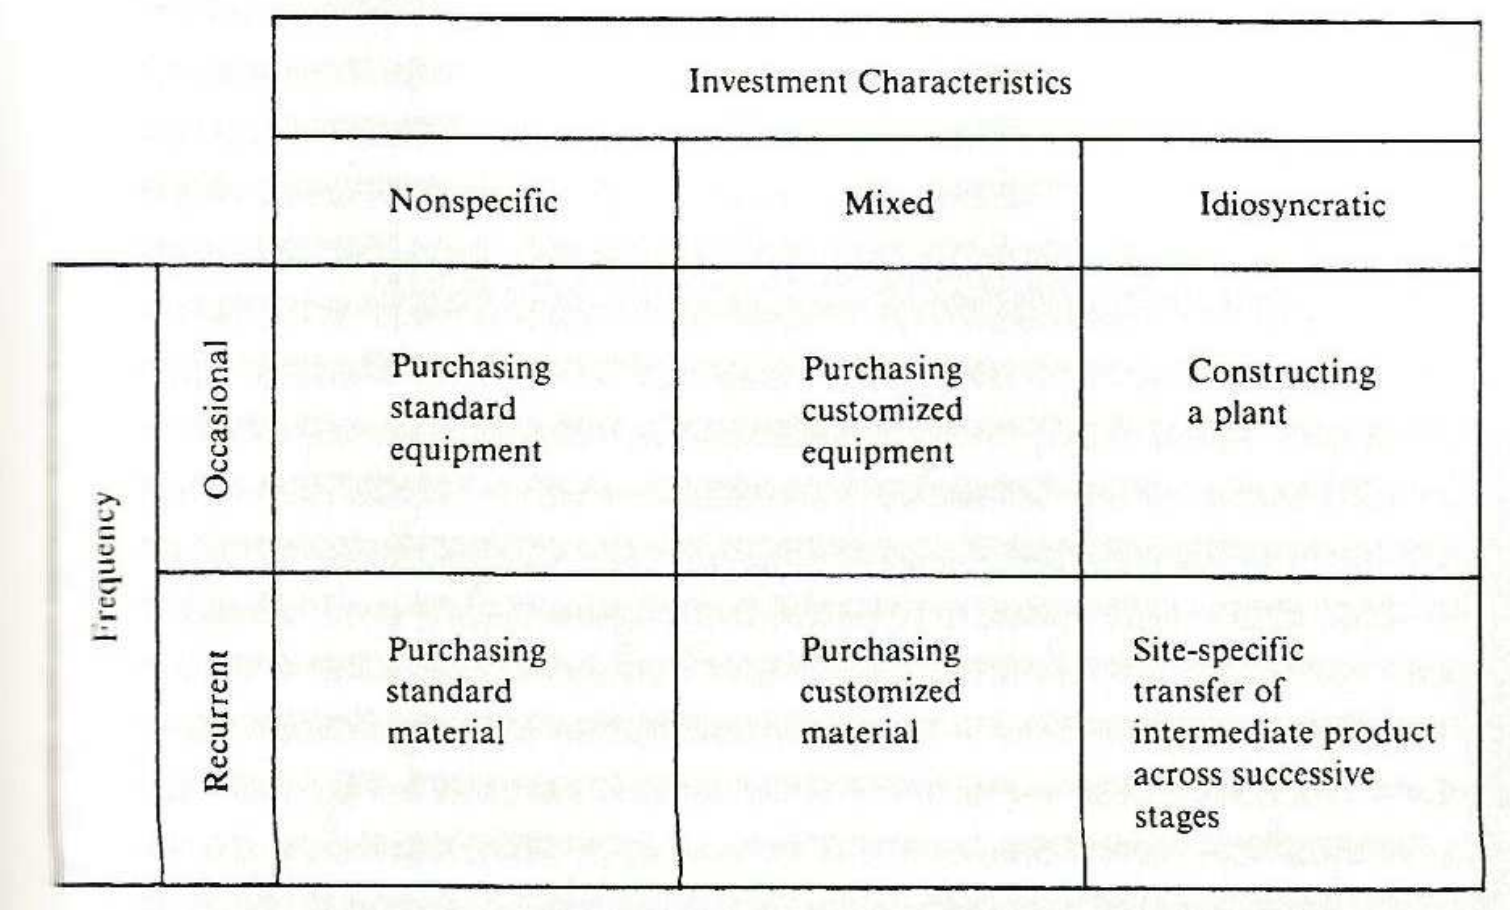
\includegraphics[width=0.7\linewidth]{screenshot006}
\end{figure}



\subsection*{Governanças eficientes}

Apesar das transações terem outras dimensões, Williamson irá focar na especificidade dos ativos e na frequência categorizados da seguinte maneira e sintetizados na tabela abaixo:

\begin{itemize}
	\item Frequência
	\begin{itemize}
		\item Única
		\item Ocasional
		\item Recorrente
	\end{itemize}
	\item Especificidade dos ativos
	\begin{itemize}
		\item Não-específicos
		\item Mistos
		\item Altamente específicos
	\end{itemize}
	\item Hipóteses simplificadoras
	\begin{itemize}
		\item Firmas temporárias podem ser desconsideradas
		\item Ofertantes potenciais são numerosos
		\item Frequência diz respeito à atividade de compra no mercado somente
		\item $\therefore$ Apenas transações ocasionais e frequentes serão consideradas e a especificidade da governança está diretamente associada tanto com a frequência quanto com a especificidade do ativo em questão
	\end{itemize}
\end{itemize}

\begin{figure}[h]
	\centering
	\caption{Governanças eficientes}
	\label{fig:screenshot007}
	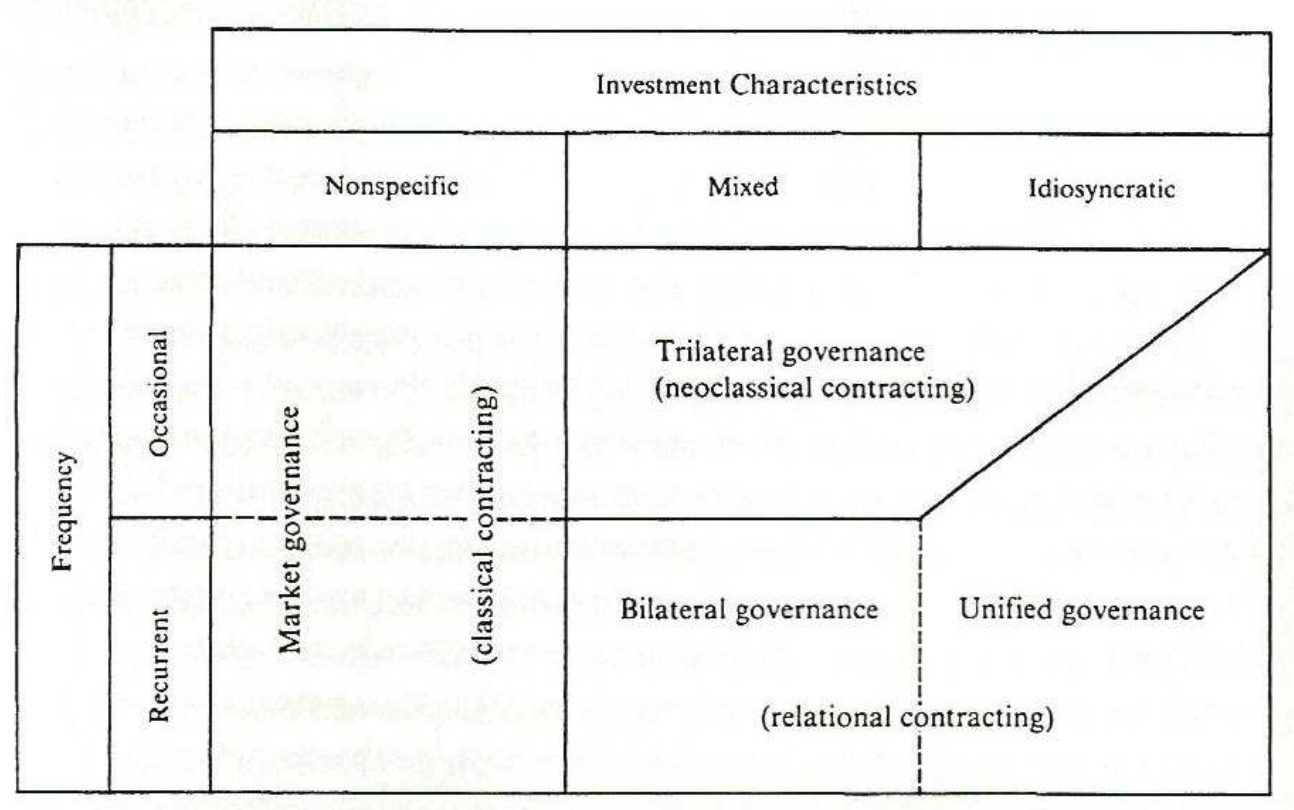
\includegraphics[width=0.7\linewidth]{screenshot007}
\end{figure}




\begin{description}
	\item[Mercado:] É a principal estrutura de governança para transações \textbf{não-específicas}, sejam elas ocasionais ou frequentes. Este tipo de transação é aquele que os contratantes estão menos aptos a se basear em suas experiências para estabelecer salvaguardar contra o comportamento oportunista. Em linhas gerais, as implicações do paradigma discreto se aplicam a esta estrutura de governança. A identidade das partes é negligenciável e o conteúdo das transações está sujeito à formalidades;
	\item[Trilateral:] São mais necessárias em transações ocasionais em que a especificidade é mista ou elevada. Sendo assim, não existem incentivos suficientes para que o contrato se dê via competição, ou seja, o mercado é insuficiente.
	\item[Bilateral:] São mais frequentes em transações frequentes cuja especificidade dos ativos é média ou elevada. Como consequência, a \textbf{transformação fundamental} ocorre por conta da natureza não convencional/padronizada das transações. Além disso, a recorrência das transações faz com que os custos elevados de uma governança especializada seja diluído. Além disso, tais estruturas preservam a \textbf{autonomia} das partes, seja pela verticalização ou relação entre-firmas. Ambas as partes têm incentivos para preservas as relações contratuais.
	\item[Unificada:] Os incentivos para as relações entre-firmas se reduzem na medida que as transações se tornam progressivamente mais específicas, ou seja, menos transferível para o uso de outros sem perdas significativas de modo que as economias de escala são realizadas por uma das partes (verticalização). A vantagem da verticalização é a menor necessidade de revisão dos contratos entre-firmas.
\end{description}

\subsection*{Incerteza}

A presença da incerteza impõe uma problema adaptativo e sequencial. Em linhas gerais, um maior grau de incerteza não afeta significativamente as transações de ativos menos específicos. No entanto, quanto maior a \textbf{especificidade dos ativos} e dada a necessidade de \textbf{continuidade} das relações contratuais, a incerteza se torna mais impositiva de modo que estruturas de governança mais adequadas são necessárias. Uma forma de lidar com a incerteza é optar por ativos menos específicos e mais usuais de modo que a governança de mercado é mais adequada. No entanto, tal especificidade pode ser preservada com uma forma de organização internalizada.

\subsection*{Mensuração}

Em linhas gerais, Williamson pontua que os problemas de governança e mensuração (ambos ramos da ECT) são negligenciáveis na ausência \textbf{tanto} de racionalidade ilimitada \textbf{quanto} de comportamento oportunista. Na ausência de racionalidade limitada, os custos de mensuração são nulos em que o comportamento oportunista invalidado. Na ausência de comportamento oportunista, a incompletude dos contratos deixa de ser um problema de governança.


\subsection*{Distribuição das transações}

Nesta seção, Williamson discute qual a ``distribuição de frequência'' dos diferentes tipos de contrato e transações. Conclui que uma distribuição \textbf{uniforme} é a que melhor descreve o mundo contratual.
\section*{Capítulo 10: A organização do trabalho}

\newcommand{\autor}{Williamson}

O autor abre o capítulo pontuando que a teoria neoclássica só passa a analisar a organização do trabalho quando se trata de uma estrutura de mercado oligopolista. A NEI, por outro lado, argumenta que a \textbf{estrutura de governança} que organiza o trabalho é relevante.

\subsection*{Questão principal}

Tal como nos demais capítulos, \autor argumenta uma teoria do contrato é aplicável a todos tipos de transação, o que inclui negociações no mercado de trabalho.

\subsection*{Uma abordagem abstrata}

A economia dos custos de transação estabelece que as estruturas de governança devem se adequar aos atributos de suas transação para que tenham efeitos de reduzir os custos de transação. O mesmo se aplica para os sindicatos e demais formas de organização laboral.

\subsubsection{Dimensões}

\begin{description}
	\item[Governança] \autor argumenta que as estruturas de governança devem ser elaboradas para dar conta do grau de especificidade do ativo (trabalho) e que as formas de negociação dependem da frequência que ocorrem. Quanto mais incerte e mais contínua é uma transação, mais terá que se adaptar.
	\item[Mensuração] \autor discute formas de medir os custos de transação e as dificuldades decorrentes da imensurabilidade da contribuição individual de cada trabalhador ao produto final. Além disso, pontua a organicidade entre os trabalhadores e as subsequentes dificuldades de substituição decorrentes dela.
	\item[Combinação provisõria] Nesta seção, \autor propõe uma forma de avaliar as estruturas de governança de acordo com a especificidade do ativo ($k_0$ e $k_1$) e separabilidade ($S_0$, $S_1$). As combinações são:
	\begin{description}
		\item[Mercado Spot ($k_0$, $S_0$)] Nem empregado ou empregador se beneficiam com a manutenção da associação
		\item[Equipe primitiva ($k_0$, $S_1$)] Por mais que os trabalhadores sejam pouco especificados, a mensuração da contribuição individual é dificultada por conta 
		\item[Mercado obrigatório ($k_1$, $S_0$)] Diz respeito à atividades específicas de cada firma cuja atividade individual é de fácil mensuração. Tanto firma quanto empregador se beneficiam da continuidade desta transação. Recomenda-se salvaguardas e penalidades pecuniárias para desestimular demissões arbitrárias
		\item[Equipe conectada ($k_1$, $S_1$)] Autoexplicativo
	\end{description}
\end{description}

\subsubsection*{Desapropriação por Trabalhadores}

\begin{description}
	\item[Ativos a serem desapropriados] Trabalhadores irão disputar as quase-rendas geradas por sua especificidade encorporada em seu capital humano. As quase-rendas potencial que podem se apropriar é determinada por seus ativos individuais
	\item[Contratos de trabalho] Resumidamente, pontua que tais contratos costumam ser mais flexíveis do que aqueles entre firmas e, portanto, existem vantagens em relação ao uso do mercado
	\item[Governança] As governanças precisam ser flexíveis a ponto de evitar riscos de desapropriação
\end{description}

\subsection*{Organização laboral}

\subsubsection*{Negociações privadas}

Nesta subseção, \autor retoma o esquema apresentado no capítulo 1 em que o tipo de transação está associado com a especificidade dos ativos. Se opta-se por uma negociação pouco específica, a estrutura de governança será simples, caso contrário, devem ser feitas escolhas de salvaguardas.

\subsubsection*{Faces de uma organização laboral}

\begin{description}
	\item[Monopólio] \autor analisa os tipos de sindicados com objetivos de aumentar salários via controle da oferta de trabalho: classe, artesanais e industriais
	\item[Eficiência] Os sindicatos podem ter propósitos de eficiência uma vez que permitem funções de agência, propor estruturas de governança, ser uma fonte de informação sobre as necessidades e preferências dos trabalhadores e auxiliar a avaliação de ofertas de trabalho. Em seguida, argumenta que o incentivo da organização laboral aumenta com a especificidade dos trabalhadores e o mesmo pode ser dito sobre forma da estrutura de governança interna. Além disso, pontua que a criação de uma unidade de governança para avaliar abusos é de interesse de ambas as partes.
	\item[Voz] Resumidamente, sindicatos são instituições políticas que representam tanto as aspirações quanto os interesses políticos de seus membros.
\end{description}

\subsubsection*{Poder}

\autor pontua a necessidade de se analisar os contratos em sua totalidade e não de forma individual e pontual. Além disso, destaca que um erro comum na literatura é avaliar o jogo de formas a partir dos ganhos de uma negociação, ou seja, de um confronto individual.

\begin{description}
	\item[Risco não diversificado] O autor pontua que o grau de não diversificação aumenta com o grau de especialização. Os trabalhadores podem escolher entre trabalhos de propósitos gerais ou específicos.
	\item[Reputação] Os custos de se encerrar uma relação contratual são dispensáveis somente em uma relação pouco específica. Ao longo do processo de contratação, os candidatos são analisados de acordo com sua reputação.
\end{description}


\subsection*{Características problemáticas da organização laboral}

\begin{description}
	\item[Poder de monopólio] Organizações laborais possibilitam os trabalhadores tenham melhores condições de barganha. Firmas com que possuem mais ativos não-humanos são mais resistentes à organização sindical.
	\item[Oligarquia] A liderança dos sindicatos, assim como a liderança de outras grandes organizações, está frequentemente em posição de se consolidar e / ou buscar interesses.
	\item[Heterogeneidade] Destaca a dificuldade de se chegar em um acordo na medida que aumenta a heterogeneidade da força de trabalho
\end{description}

\subsection*{Conclusões}


\begin{itemize}
	\item Estruturas de governança especializadas são dispensáveis em transações de trabalho pouco específicas. Caso surjam, as uniões laborais surgirão tardiamente
	\item Mercado de trabalho especializado e sem salvaguardas está sujeito à expropriações e não é estável
	\item Mercados especializados e com salvaguardas são aqueles que organizações coletivas são mutuamente acordadas uma vez que ambas as partes se beneficiam dela. As estruturas de governança possuem maior grau de elaboração
\end{itemize}


\begin{sigstatement}
	\sffamily
	\mdfdefinestyle{stylesigstyle}{linewidth=0.7pt,
		backgroundcolor=styleblueback,linecolor=stylebluetext,
		fontcolor=stylebluetext,innertopmargin=6pt,innerrightmargin=6pt,
		innerbottommargin=6pt,innerleftmargin=6pt}
	{%	
		\begin{mdframed}[style=stylesigstyle]%
			\section*{Dúvidas}%
			Na página 23, Williamson (1987) afirma:
			\begin{quotation}
				\textit{Wheneverprivate and social benefits and costs differ, the social cost
					calculus should govern if prescriptive treatments are attempted.}
			\end{quotation}
			O que seriam esses \textit{prescriptive treatments}? 
			
	\end{mdframed}}
\end{sigstatement}
	
\end{document}